\section{Flag 08 - File Upload}

\paragraph{46910d9ce35b385885a9f7e2b336249d622f29b267a1771fbacf52133beddba8}

\begin{center}
    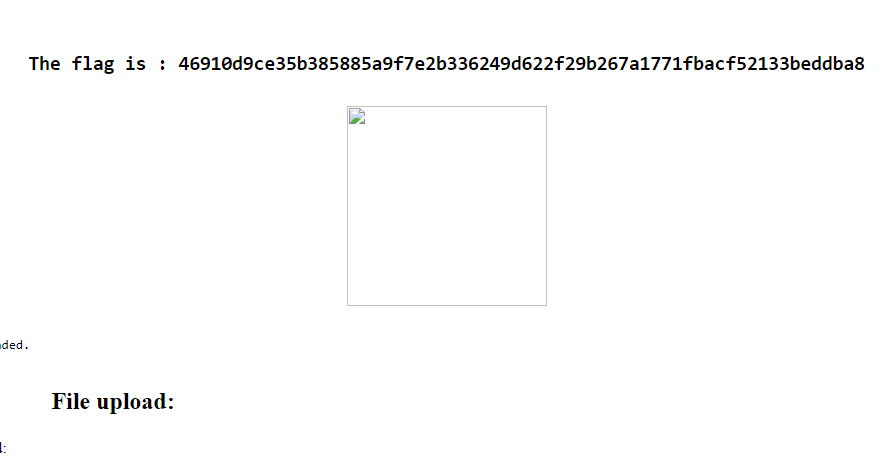
\includegraphics[width=0.5\textwidth]{11.Flag08/08-03.png}\\[0cm] 
\end{center}

\subsection{Vulnerability}

Uploaded files represent a significant risk to applications. The first step in many attacks is to get some code to the system to be attacked. Then the attack only needs to find a way to get the code executed. Using a file upload helps the attacker accomplish the first step.

\subsection{Location}

http://<ip-address>:80/index.php?page=upload\#

\subsection{Method}

When one opens the upload, you will see from Inspecting that the page has a POST method.

You must also note that it uses nginx, not apache, which is susceptible to double extension attacks. So file.sh.jpg would not work.

You will see the MAX\_FILE\_SIZE is set on the front, which is bad but to test, I also tried to upload a large file, I received a 413 Error.

When we continue to examine the page, we see that the `name` of the upload is `uploaded`. So the aim is to try breach the upload using a cURL.

It is easy to create a cURL script, the one I made is this:

```

ip="http://<ip-address>"

curl -o sinkosi.html -X POST \\

-F 'Upload=Upload' \\

-F 'uploaded=@file.php;type=image/jpeg' \\

"\${ip}/?page=upload"

```

- -X POST: Tells curl we are making a post request method
- -F 'Upload=Upload': tells curl we are making an upload to an object named upload.
- @: Force the content
-o sinkosi.html: Output the result to sinkosi.html

When the curl has run, open sinkosi.html, the flag will be posted there.


\subsection{Tools}

\begin{figure}[!htb]
    \centering
    \subfloat[Link Location]{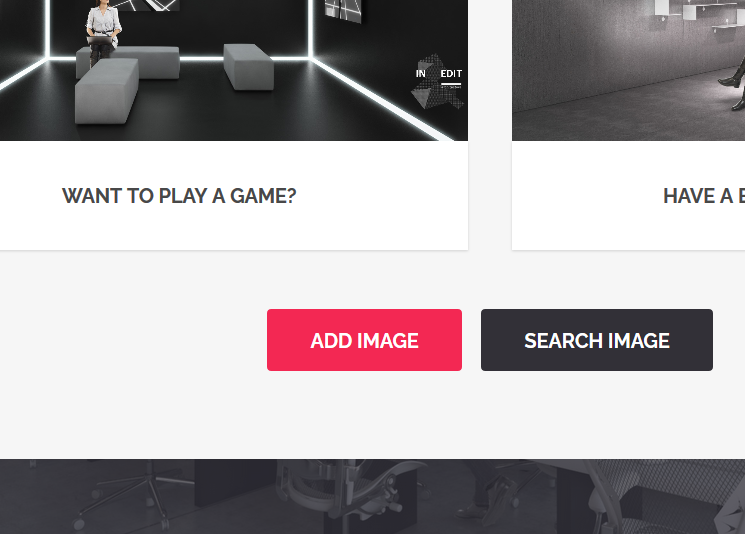
\includegraphics[width=.45\columnwidth]{11.Flag08/08-01.png}\label{fig: 08-01 - wtf}} \quad
    \subfloat[FIle Upload]{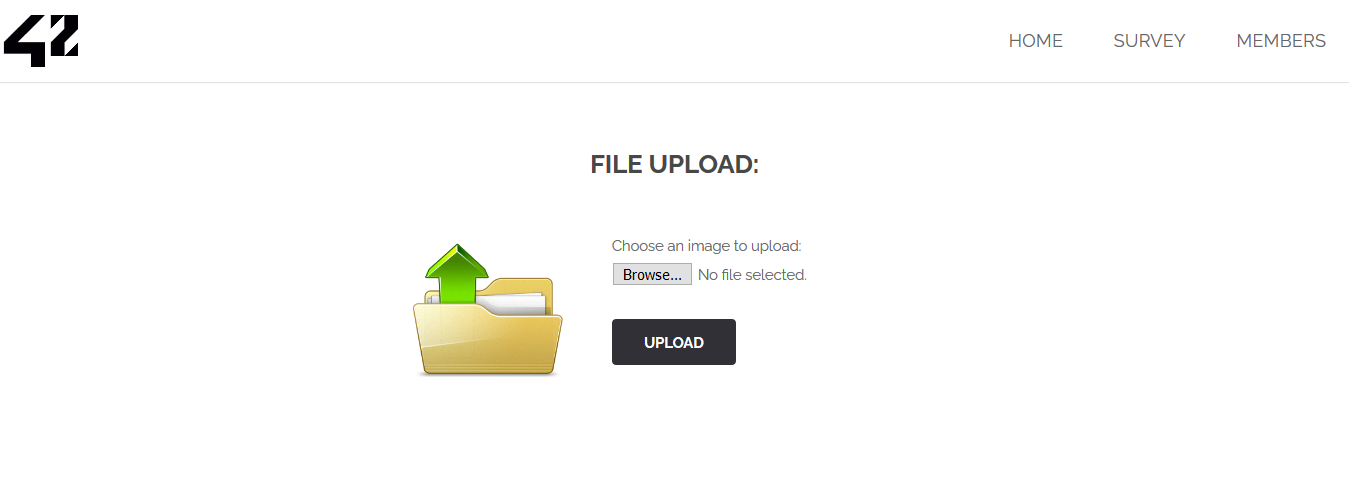
\includegraphics[width=.45\columnwidth]{11.Flag08/08-02.png}\label{fig: 08-02 - wrong}} \\
    \caption[Flag 08 Method]{Process to Capture the File Upload Flag} % The text in the square bracket is the caption for the list of figures while the text in the curly brackets is the figure caption
    \label{fig:flag08 method}
\end{figure}

\begin{itemize}
    \item \href{https://owasp.org/www-community/vulnerabilities/Unrestricted_File_Upload}{OWASP}
    \item \href{https://medium.com/@petehouston/upload-files-with-curl-93064dcccc76}{Medium}
\end{itemize}

\subsection{Remedy}

\begin{itemize}
    \item Limit the filename length. For instance, the maximum length of the name of a file plus its extension should be less than 255 characters (without any directory) in an NTFS partition.
    \item It is recommended to use an algorithm to determine the filenames. For instance, a filename can be a MD5 hash of the name of file plus the date of the day.
    \item Uploaded directory should not have any “execute” permission and all the script handlers should be removed from these directories.
    \item Limit the file size to a maximum value in order to prevent denial of service attacks (on file space or other web application’s functions such as the image resizer).
    \item Restrict small size files as they can lead to denial of service attacks. So, the minimum size of files should be considered.
    \item Use Cross Site Request Forgery protection methods.
    \item Prevent from overwriting a file in case of having the same hash for both.
    \item Ensure that files with double extensions (e.g. “file.php.txt”) cannot be executed especially in Apache.
    \item Ensure that uploaded files cannot be accessed by unauthorised users.
    \item Adding the “Content-Disposition: Attachment” and “X-Content-Type-Options: nosniff” headers to the response of static files will secure the website.
    \item CORS headers should be reviewed to only be enabled for static or publicly accessible data. Otherwise, the “Access-Control-Allow-Origin” header should only contain authorised addresses. Other CORS headers such as “Access-Control-Allow-Credentials” should only be used when they are required. Items within the CORS headers such as “Access-Control-Allow-Methods” or “Access-Control-Allow-Headers” should be reviewed and removed if they are not required.
\end{itemize}
